\documentclass[a4paper,11pt,dvipdfmx]{ujarticle}

\usepackage{graphicx}
\usepackage{url}
\input{layout}

% タイトルと氏名を変更せよ.
\title{日本におけるデジタル化の状況}

\author{G58499-2025 山本 真大}

\begin{document}

\maketitle 

\section{ブロードバンドの整備状況}

OECDによるブロードバンド回線の普及に関する調査\cite{oecd}によると、図\ref{fig:1}に示すように、
日本における100人あたりのモバイルブロードバインドの加入者数は190.5で、第1位になっている。
2位はエストニアで、3位米国と続く。

\begin{figure}[htbp]
    \centering
    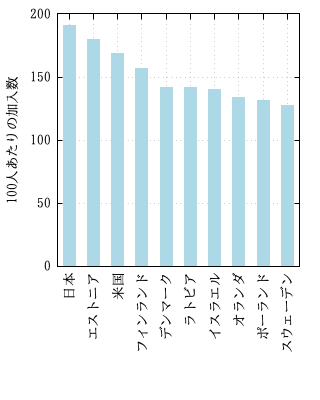
\includegraphics[width=0.5\linewidth]{img2.png}
    \caption{光ファイバー回線の加入者数(100人あたり)}\label{fig:1}
\end{figure}

\section{デジタル競争ランキング}

国際経営開発研究所(IMD)の調査\cite{imd}によると、
日本のデジタル競争力のランキングは表\ref{tbl:デジタル}に示すように、
調査対象の64カ国中、総合で28位、技術分野で30位になっている。

\begin{table}[htbp]
    \centering
    \caption{デジタル競争力ランキング(64カ国中)}
    \label{tbl:デジタル}

    \begin{tabular}{|c|r|r|}\hline
        国 & 総合 & 技術 \\
        \hline
        米国 & 1位 & 4位 \\
        \hline
        香港 & 2位 & 10位 \\
        \hline
        スウェーデン & 3位 & 8位 \\
        \hline
        デンマーク & 4位 & 2位 \\
        \hline
        シンガポール & 5位 & 3位 \\
        \hline
        \hline
        韓国 & 12位 & 13位 \\
        \hline
        中国 & 15位 & 20位 \\
        \hline
        \hline
        日本 & 28位 & 30位 \\
        \hline
    \end{tabular}
\end{table}

\section{考察}

\begin{itemize}
    \item  日本はモバイルブロードバンド加入者数が1位
    \item  モバイルブロードバンド加入者は日本とスウェーデンでは約100の差がある
    \item  日本のデジタル競争力が総合で30位と低い
    \item  米国がデジタル競争力が高い
\end{itemize}


%ここにタイトルが入る
% ここから本文
% 節見出し: \section{}
% を使う
% 本文(1)
%  参考文献の参照: \cite{}
%  図番号の参照: \ref{}
% を使う
% 文献データベースのキーワードは oecd と imd
% になっている.

% 図の挿入
% \includegraphics{}
% を
% \begin{figure}[htbp]
% \end{figure}
% で囲み
% \caption{}
% で図のタイトルを入れる.
% \label{}
% を使って図番号が参照できるようにする
% また,
% \centering
% で図が中央に来るようにする

% ーーー
% 節見出し(2)

% 本文(2)

% 表の挿入
% \begin{tabular}
% \end{tabular}    
% による表の記述を 
% \begin{table}[htbp]
% \end{table}
% で囲み
% \caption{}
% で表のタイトルを入れる.
% \label{}
% を使って表番号が参照できるようにする
% また,
% \centering
% で表が中央に来るようにする

% ーーー
% 見出し(3)
% 考察
%
% \begin{itemize}
% \end{itemize}
% を使って箇条書きで記述する

% ここに参考文献が入る
%
\bibliographystyle{junsrt}
\bibliography{exercise.bib}

\end{document}